\chapter{Interface Overview}
\begin{figure}[H]
\centering
  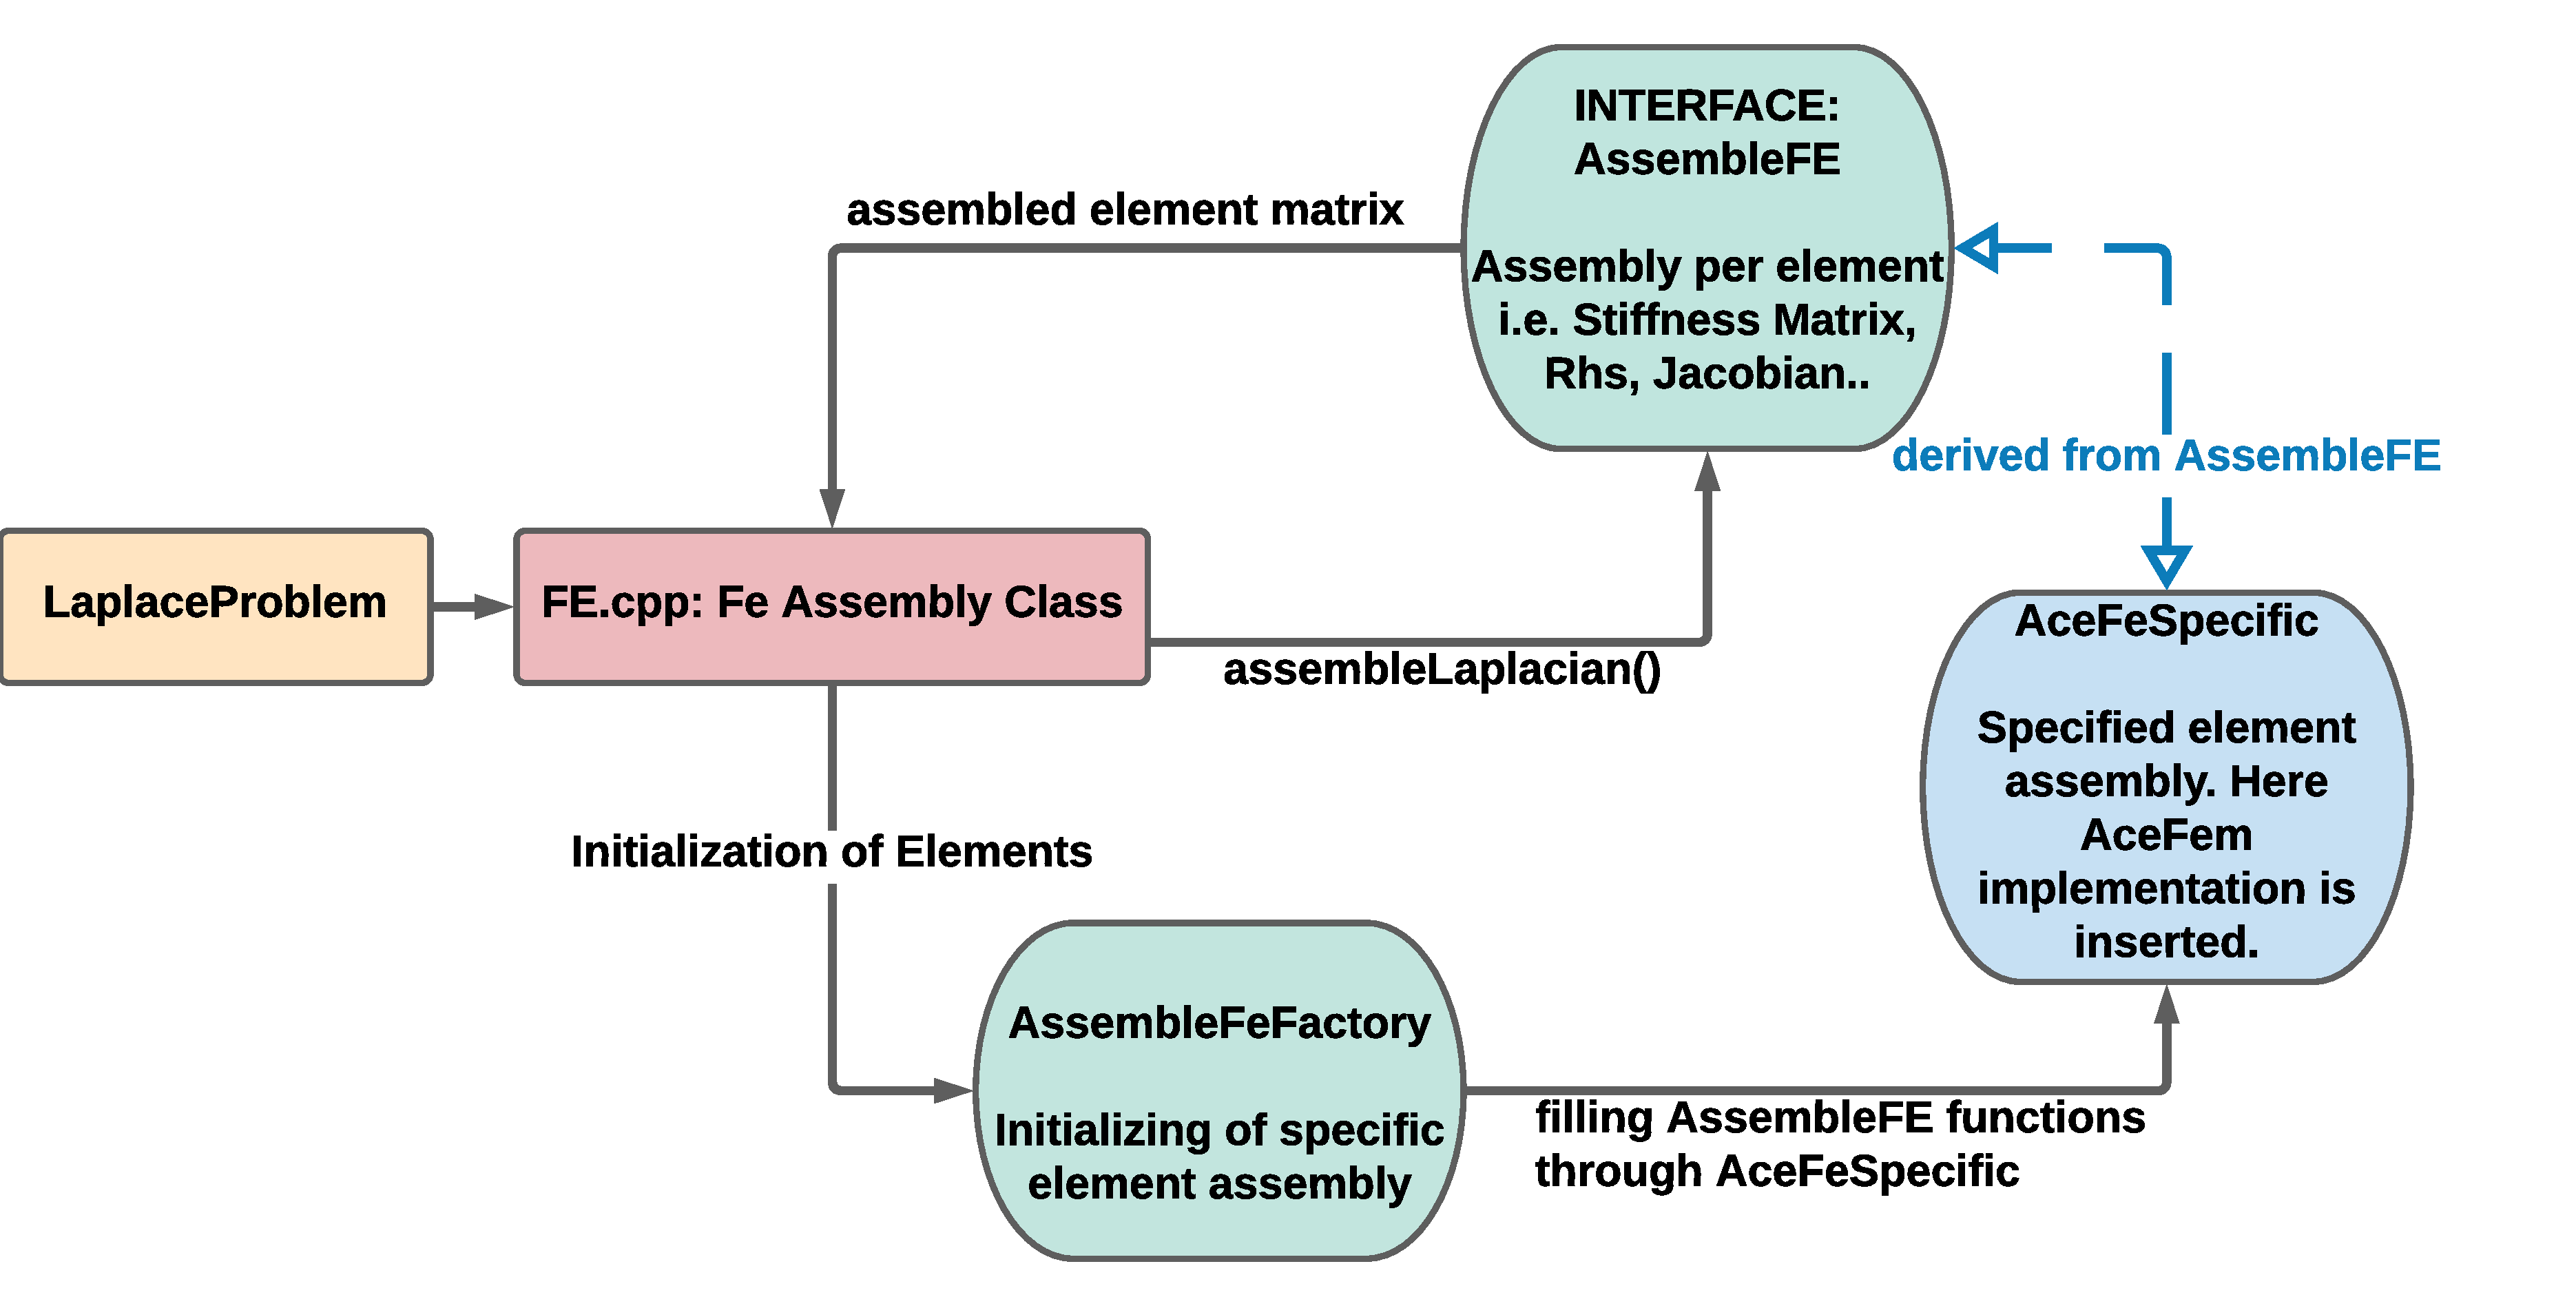
\includegraphics[width=1\textwidth , height=0.5\textwidth]{AceFe.pdf}
 \caption{Accessing AceFem Implementation. Example for assembling finite element stiffness matrix for Laplace problem.}
\end{figure}

For implementing the interface we need three new classes:
\begin{itemize}
\item \texttt{AssembleFE}
\item \texttt{AssembleFEFactory}
\item \texttt{AceFeSpecific}
\end{itemize}

\section{\texttt{AssembleFE} Class}
\texttt{AssembleFE} is the basis class and interface for the finite element assembly.\\
We access the \texttt{AssembleFE} Implementation in the general finite element assembling class \texttt{FE}.

$\rightarrow$ For each element we should be able to assemble different finite element entities, for example stiffness matrix, right hand side or Jacobian matrix, with the \texttt{AssembleFE} object.
\begin{lstlisting}
// Assembly of element matrix for laplacian operator
AssembleFE.assemblyLaplacian(); 
\end{lstlisting}
\captionof{lstlisting}{Calling \texttt{assemblyLaplacian()} of \texttt{AssembleFE} in \texttt{FE.cpp}}
~~\\
The \texttt{AssembleFE} class only owns virtual assembling functions.
\begin{lstlisting}
virtual void assemblyLaplacian() = 0;
virtual void assemblyRHS() = 0;
\end{lstlisting}
\captionof{lstlisting}{An example of virtual assembly functions of \texttt{AssembleFE}.}
~~\\
Those virtual functions are initialized through \texttt{AssembleFEFactory} with the corresponding \texttt{AceFeSpecific} assembly functions.

As an \texttt{AssembleFE} object represents one element, the implementation within \texttt{AssembleFE} is independent of any parallel implementation. The \texttt{FE} class distributes the local element matrices to the global matrices accordingly.

\section{\texttt{AssembleFEFactory} Class}
The \texttt{AssembleFEFactory} class fills the virtual functions of \texttt{AssembleFE} with the corresponding functions of the specific problem.
It builds the \texttt{AceFeSpecific} object of the \texttt{AssembleFE} basis object. 
\begin{lstlisting}
AssembleFEFactory(string problemType, AssembleFE_Type assembleFE ):
{
if(problemType == "Laplace"){
	assembleFE = new AceFeSpecificLaplace();
}
else if( ..)

}
\end{lstlisting}
\captionof{lstlisting}{Constructor of \texttt{AssembleFEFactory} that initializes the \texttt{assembleFE} object.}

\section{\texttt{AceFeSpecific} Class}

The \texttt{AceFeSpecific} class is derived from \texttt{AssembleFE} and extends the virtual functions with specific assembly rules.
Each specific problem corresponds to a \texttt{AceFeSpecific} class of functions. 

For a Laplace problem we would have a \texttt{AceFeSpecificLaplace} class with its corresponding assembly of right hand side and stiffness matrix (see Code \ref{CodeLaplace}).
 ~~\\
 
For adding a new element or assembly routine (or \textbf{AssembleFem} code), one must simply add a new or extend an \texttt{AceFeSpecific} class that fulfills \texttt{AssembleFE}'s assembly  requirements and add the build information to \texttt{AssembleFEFactory}. This way the element assembly can be accessed equally in the \texttt{FE} class for each specific assembly routine that is concealed in the \texttt{AceFeSpecific} classes. 
 ~~\\
 ~~\\
 ~~\\
\begin{lstlisting}
void assemblyLaplacian(Matrix &ElementMatrix){
	
    numNodes= nodesRefConfig_.size(); // number of nodes per element
    dPhi = this->getDPhi(dim_, FEType_); // nabla phi
    Matrix B(dim_); // transformation matrix
    Matrix Binv(dim_); // inverse of transformation matrix
    this->buildTransformation(B); // building inverse
    detB = B.computeInverse(Binv);  // determinent of inverse
    dPhiTrans = this->applyBTinv( dPhi,Binv ); // applying inverse to dPhi
    
    // Filling element matrix with correct values
    for (int i=0; i < numNodes; i++) {
        for (int j=0; j < numNodes; j++) {
            ElementMatrix[i][j] = //assembly rules; 
        }
    }
}
\end{lstlisting}
\captionof{lstlisting}{\texttt{AssemblyLaplacian()} in \texttt{AceFeSpecificLaplace}. }
\label{CodeLaplace}


%\newpage
%\section{Open Questions}
%\begin{itemize}
%\item How specific are the assembly functions?
%\item Where are basis functions, quadrature values and other useful functions stored (i.e. buildTransformation)?
%\item How exactly is the AceFeFactory build process of AceFeSpecific?
%\item What is the Output of assembly? Input\/Output Point or return value?
%\end{itemize}
%
%\chapter{Interface in Detail}
%
%\section{Basisclass}
%
%
%\textbf{The following functions are not uniquely defined for different problems and thus are not virtual functions, but implemented in \texttt{AceFe}}?
%\begin{lstlisting}[caption=Additional Functions and Features]
%updateSolution(); // i.e. for nonlinear iterations
%
%initParams(); // initializing important assembly params
%updateParams(); // updating parameters in case its needed
%
%advanceInTime(); // signaling advancement in time
%
%preProcessing(); //
%postProcessing(); //
%\end{lstlisting}
%
%Each \texttt{AceFe} element holds detailed information of the current problem.
%\begin{lstlisting}[caption=Variables]
%private:
%	string FEType_; // Finite Element discretization
%	int dim_; // Dimension
%	int dofs_; // Degrees of freedom
%	const int numNodes_; // Number of nodes (of element)
%	vec2D_dbl_Type nodesRefConfig_; // Nodes	
%	vec_dbl_Type paramsMaterial_; // Material Parameters
%	bool timeProblem_; // Time dependent problem
%	int flag_; // Element Flag
%	...
%\end{lstlisting}
